\documentclass[10pt,dvipdfm]{beamer}

\usepackage{color}
\usepackage{amsmath}
\usepackage{amssymb}
\usepackage{mathrsfs}
\usepackage{tikz}

\newtheorem{proposition}{Proposition}
\newtheorem{remark}{Remark}


\everymath{\displaystyle}

\newcommand{\CC}{\mathbb{C}}

\title{量子群と\\ヤン・バクスター\\方程式}
\author{つばきちゃん}

\begin{document}
  \begin{frame}
    \titlepage
  \end{frame}
  \begin{frame}
    \frametitle{目次}
    \tableofcontents
  \end{frame}
  \subsection{可換性・余可換性}
  \begin{frame}
    \frametitle{可換性・余可換性}
    双代数やホップ代数が可換であるとは単に代数として可換であるということである.

    双代数$(H,m,n,\Delta,\varepsilon)$に対して$(H,m,n,\Delta',\varepsilon)$もまた双代数であることは容易に示される.

    さらに$H$が対合射$S$を持ち,$S$が可逆であるとすると,
    \begin{align*}
      \sum a^{(1)}S^{-1}(a^{(2)}) &= \sum S(S^{(-1)}(a^{(1)}))S^{-1}(a^{(2)}) \\
      &= \varepsilon(a)1_H\\
      \sum S^{-1}(a^{(1)})a^{(2)} &= \sum S^{-1}(a^{(1)})S(S^{(-1)}(a^{(2)})) \\
      &= \varepsilon(a)1_H\\
      \Delta'(a) &= \sum a^{(2)}\otimes a^{(1)}
    \end{align*}
    この結果は$(H,m,n,\Delta',\varepsilon)$がホップ代数であることを示している.
  \end{frame}
  \begin{frame}
    \begin{definition}
      余代数,双代数,ホップ代数が余可換であるとは,$\Delta' = \Delta$が成り立つことをいう.
    \end{definition}
    ここで例$1.8$のホップ代数$H$は可換である.
    
    $H$の積$m$は$\varphi\in H\otimes H(\in G\times G \to \CC)$に対して
    \[
    m(\varphi)(x) = \varphi(x,x)
    \]
    と定義される.
    このとき$\varphi'(a,b)=\varphi(b,a)$を考えると
    \[
    m(\varphi')(x) = \varphi'(x,x) = \varphi(x,x) = m(\varphi)(x)
    \]
  \end{frame}
  \begin{frame}
    また,$f \in H (\in G \to \CC)$に対して$\Delta(f)(x,y) = f(xy)$であり,
    $\Delta'(f)(x,y) = f(yx)$であるので,$H$が余可換$(\Delta=\Delta')$であるということは,
    $f(xy) = f(yx)$が成り立つことをいう.

    つまり$H$が余可換であるとは$G$が可換であることをいう.

    包絡環$U(\mathfrak{g})$について$U(\mathfrak{g})$が可換であるとき,
    $AB=BA$となり,$[A,B]=0$が成り立たなくてはならない.
    つまり$\mathfrak{g}$は可換となる.
  \end{frame}
  \begin{frame}
    余可換なホップ代数について余代数$C$が単純であるとは,
    $C$と$0$以外の部分余代数を持たないことをいう.

    ただ$1$つの単純部分余代数を持つとき,$C$を既約であるという.
    \begin{theorem}
      既約余可換なホップ代数$H$について,あるリー環$\mathfrak{g}$が存在して$H\simeq U(\mathfrak{g})$となる.
    \end{theorem}
  \end{frame}
  \section{$U_q(\mathfrak{sl}(2,\CC))$}
  \begin{frame}
    リー環$\mathfrak{sl}(2,\CC)$に付随する量子包絡環$U_q(\mathfrak{sl}(2,\CC))$を考える.
    まず$\mathfrak{sl}(2,\CC)$を定義する.
    \begin{definition}
      \begin{align*}
        \mathfrak{sl}(2,\CC) &= \{X \in \text{Mat}(2,\CC) | \text{tr} X = 0\}
      \end{align*}
      ベクトル空間として$\mathfrak{sl}(2,\CC)$は基底
      \[
      E=\begin{pmatrix} 0 & 1 \\ 0 & 0 \end{pmatrix},\quad F=\begin{pmatrix} 0 & 0 \\ 1 & 0 \end{pmatrix},\quad H=\begin{pmatrix} 1 & 0 \\ 0 & -1 \end{pmatrix}
      \]
      を持つ.
    \end{definition}
    交換関係$[A,B]=AB-BA$について,基底$E,F,H$は,
    \[
    [H,E]=2E,\quad [H,F]=-2F,\quad [E,F]=H
    \]
    が成り立つ.
  \end{frame}
  \begin{frame}
    量子包絡環$U_q(\mathfrak{sl}(2,\CC))$は$U(\mathfrak{sl}(2,\CC))$の$q$版である.
    ここで$q$は$0,\pm1$ではない任意の複素数である.

    量子包絡環$U_q(\mathfrak{sl}(2,\CC))$は$X^+,X^-,K,K^{-1}$で,生成される自由結合代数で,
    次の関係式を満たすものである.
    \begin{align*}
      KK^{-1} &= K^{-1}K = 1\\
      KX^{\pm}K^{-1} &= q^{\pm2}X^{\pm}\\
      [X^+,X^-] &= \frac{K-K^{-1}}{q-q^{-1}}
    \end{align*}
    このことを詳しく述べると,
    $X^+,X^-,K,K^{-1}$を基底に持つベクトル空間上の自由結合代数$\mathscr{J}$を
    イデアル$\mathscr{I}$で割ったものが$U_q(\mathfrak{sl}(2,\CC))$である.
    $\mathscr{I}$は
    \[
    KK^{-1}-1,\quad K^{-1}K-1,\quad KX^{\pm}K^{-1}-q^{\pm2}X^{\pm},\quad [X^+,X^-]-\frac{K-K^{-1}}{q-q^{-1}}
    \]
    で生成される.
  \end{frame}
  \begin{frame}
    リー環$\mathfrak{sl}(2,\CC)$と比較してみる.

    その準備として次の定理を示す.
    \begin{theorem}
      リー環の不定元$A,B$に対して
      リー括弧$[A,-]$を$B$に$n$回作用させることを$[A,B]_n$と書く.
      このとき,$[A,B]_n=\sum_{k=0}^{n}\binom{n}{k}A^{n-k}B(-A)^k$である.
    \end{theorem}

  \end{frame}
  \begin{frame}
    \begin{proof}
      $n=0$のとき,
      \[
      \sum_{k=0}^{0}\binom{0}{k}A^{0-k}B(-A)^k = B = [A,B]_0
      \]
      となる.
      $n>0$のとき,
      \[
      [A,B]_n = \sum_{k=0}^{n}\binom{n}{k}A^{n-k}B(-A)^k
      \]
      が成り立つとすると,
      \let\qedsymbol\relax
    \end{proof}
  \end{frame}
  \begin{frame}
    \begin{proof}
      \begin{align*}
        &[A,[A,B]_n]\\ 
        &= [A,\sum_{k=0}^{n}\binom{n}{k}A^{n-k}B(-A)^k]\\
        &= \sum_{k=0}^{n}\binom{n}{k}A^{n-(k - 1)}B(-A)^k + \sum_{k=0}^{n}\binom{n}{k}A^{n-k}B(-A)^{k+1}\\
        &= \sum_{k=0}^{n}\binom{n}{k}A^{n-(k - 1)}B(-A)^k + \sum_{k=1}^{n+1}\binom{n}{k-1}A^{n-(k-1)}B(-A)^{k}\\
        &= \binom{n}{0} A^{n+1}B + \sum_{k=1}^{n}\left(\binom{n}{k}+\binom{n}{k-1}\right)A^{n-(k+1)}B(-A)^k + \binom{n}{n}B(-A)^{n+1}\\
        &= \binom{n+1}{0} A^{n+1}B + \sum_{k=1}^{n}\binom{n+1}{k}A^{n+1-k}B(-A)^k + \binom{n+1}{n+1}B(-A)^{n+1}\\
        &= \sum_{k=0}^{n+1}\binom{n+1}{k}A^{n+1-k}B(-A)^k = [A,B]_{n+1}
      \end{align*}
    \end{proof}
  \end{frame}
  \begin{frame}
    これにより,$e^{\varepsilon A}Be^{-\varepsilon A}$は
    \begin{align*}
      e^{\varepsilon A}Be^{-\varepsilon A} &= \sum_{k=0}^{\infty}\frac{\varepsilon A}{k!} B \sum_{l=0}^{\infty}\frac{(-\varepsilon A)^l}{l!} \\
      &= \sum_{k=0}^{\infty}\sum_{l=0}^{\infty}\frac{\varepsilon^k(-\varepsilon)^l}{k!l!}A^kB(-A)^l\\
      &= \sum_{k=0}^{\infty}\sum_{l=0}^{\infty}\frac{(-1)^l\varepsilon^{k+l}}{k!l!}A^kB(-A)^l
    \end{align*}
    ここで,$m=k+l$とする.
    \begin{align*}
      &= \sum_{m=0}^{\infty}\sum_{l=0}^{m}\frac{(-1)^l\varepsilon^{m}}{l!(m-l)!}A^{m-l}B(-A)^l \\
      &= \sum_{m=0}^{\infty}\frac{\varepsilon^{m}}{m!}\sum_{l=0}^{m}\binom{m}{l}A^{m-l}B(-A)^l \\
      &= \sum_{m=0}^{\infty}\frac{\varepsilon^{m}}{m!}[A,B]_m
    \end{align*}
  \end{frame}
  \begin{frame}
    $\sum_{k=0}^{\infty}\sum_{l=0}^{\infty}\frac{(-1)^l\varepsilon^{k+l}}{k!l!}A^kB(-A)^l$の絶対収束性について
    \begin{align*}
      \sum_{k=0}^{\infty}\sum_{l=0}^{\infty}\left|\frac{(-1)^l\varepsilon^{k+l}}{k!l!}A^kB(-A)^l\right| &= \sum_{k=0}^{\infty}\sum_{l=0}^{\infty}\frac{|\varepsilon|^{k+l}}{k!l!}|A|^k|B||A|^l\\
      &= |B| \sum_{k=0}^{\infty}\frac{|\varepsilon|^k}{k!}|A|^k \sum_{l=0}^{\infty}\frac{|\varepsilon|^l}{l!}|A|^l\\
      &= |B|e^{|\varepsilon||A|}e^{|\varepsilon||A|} = |B|e^{2|\varepsilon||A|}
    \end{align*}

    となり,絶対収束する.

    つまり先の順序交換が成立する.
  \end{frame}
  \begin{frame}
    ここで$A=H,B=E,q=e^{\varepsilon}$とすると,
    $e^{\varepsilon A}Be^{-\varepsilon A}=\sum_{m=0}^{\infty}\frac{\varepsilon^{m}}{m!}[A,B]_m$は
    \begin{align*}
      q^H E q^{-H} &= \sum_{m=0}^{\infty}\frac{\varepsilon^{m}}{m!}[H,E]_m\\
      &= \sum_{m=0}^{\infty}\frac{(2\varepsilon)^{m}}{m!}E\\
      &= e^{2\varepsilon}E\\
      &= {e^{\varepsilon}}^2 E\\
      &= q^2 E
    \end{align*}
    この関係により,$K = q^H,X^+=E,X^-=F$とおき,$\mathfrak{sl}(2,\CC)$の交換関係を書き直したものであるといことがわかる.

    本質的に$U_q(\mathfrak{sl}(2,\CC))$と$\mathfrak{sl}(2,\CC)$はが異なる点は,
    リー括弧$[A,B]$の関係式のみである.
    しかし,$q\to1$の極限で$[X^+,X^-]=\frac{K-K^{-1}}{q-q^{-1}}$は$[E,F]=H$に還元される.
  \end{frame}
  \subsection{ホップ代数の構造}
  \begin{frame}
    以下$U_q = U_q(\mathfrak{sl}(2,\CC))$とする.

    $U_q$についてホップ代数の構造を考える.
    まず$U_q$の生成元$X^+,X^-,K,K^{-1}$に対して,次の関係式を定義する.
    \begin{align*}
      \Delta(K^{\pm1}) &= K^{\pm1}\otimes K^{\pm1}\\
      \Delta(X^+) &= X^+\otimes 1 + K\otimes X^+\\
      \Delta(X^-) &= X^-\otimes K^{-1} + 1\otimes X^-\\
      \varepsilon(K^{\pm1}) &= 1\\
      \varepsilon(X^{\pm}) &= 0\\
      S(K^{\pm1}) &= K^{\mp1}\\
      S(X^+) &= -K^{-1}X^+\\
      S(X^-) &= -X^-K
    \end{align*}
    $U_q$全体には$\Delta,\varepsilon$を代数射として,
    $S$を反代数射として拡張する.
  \end{frame}
  \begin{frame}
    \begin{proposition}
      $\Delta,\varepsilon$ は$U_q$上の代数射としてWell-definedである.
    \end{proposition}
    \begin{proof}
      $\mathscr{J}$において$\Delta,\varepsilon$を代数射として拡張することができる.

      $a,b\in\mathscr{J}$に対して$a\sim B\leftrightarrow a-b\in\mathscr{I}$であり,
      $a\sim b$ならば$\Delta(a)\sim\Delta(b),\varepsilon(a)=\varepsilon(b)$が成り立つことを確認する.
      
      $a\sim b$に対して
      \[
      \Delta(a)-\Delta(b) = \Delta(a-b)
      \]
      $a-b\in \mathscr{I}$であるので$x \in \mathscr{I}$として$\Delta(x)=0$を示す.
      \begin{align*}
        x =& a(KK^{-1}-1)+b(K^{-1}K-1)+c(KX^+K^{-1}-q^+X^+)\\
        &+d(KX^-K^{-1}-q^-X^-)+e\left([X^+,X^-]-\frac{K-K^{-1}}{q-q^{-1}}\right)\\
        \Delta(x) =& a\Delta(KK^{-1}-1)+b\Delta(K^{-1}K-1)+c\Delta(KX^+K^{-1}-q^+X^+)\\
        &+d\Delta(KX^-K^{-1}-q^-X^-)+e\Delta\left([X^+,X^-]-\frac{K-K^{-1}}{q-q^{-1}}\right)
      \end{align*}
      \let\qedsymbol\relax
    \end{proof}
  \end{frame}
  \begin{frame}
    \begin{proof}
      \begin{align*}
        \Delta(KK^{-1}-1) &= \Delta(K)\Delta(K^{-1}) - \Delta(1)\\
        &= (K\otimes K)(K^{-1}\otimes K^{-1}) - 1\otimes 1\\
        &= KK^{-1}\otimes KK^{-1} - 1\otimes 1\\
        &= 1\otimes 1 - 1\otimes 1 = 0
      \end{align*}
      となり,同様に$\Delta(K^{-1}K-1)=0$
      \begin{align*}
        \Delta&(KX^+K^{-1}-q^2X^+)\\ 
        &= \Delta(K)\Delta(X^+)\Delta(K^{-1}) - q^2\Delta(X^+)\\
        &= (K\otimes K)(X^+\otimes 1 + K\otimes X^+)(K^{-1}\otimes K^{-1}) - q^2(X^+\otimes 1 + K\otimes X^+)\\
        &= KX^+K^{-1}\otimes 1 + K\otimes KX^+K^{-1} - q^2(X^+\otimes 1 + K\otimes X^+)\\
        &= q^2X^+\otimes 1 + K\otimes q^2X^+ - q^2(X^+\otimes 1 + K\otimes X^+)\\
        &= q^2(X^+\otimes 1 + K\otimes X^+) - q^2(X^+\otimes 1 + K\otimes X^+) = 0
      \end{align*}
      となり,同様に$\Delta(KX^-K^{-1}-q^{-2}X^-)=0$となる.
      \let\qedsymbol\relax
    \end{proof}
  \end{frame}
  \begin{frame}
    \begin{proof}
      \begin{align*}
        &\Delta\left([X^+,X^-] - \frac{K-K^{-1}}{q-q^{-1}}\right) \\
        &= \Delta\left(X^+X^- - X^-X^+ - \frac{K-K^{-1}}{q-q^{-1}}\right)\\
        &= \Delta(X^+)\Delta(X^-) - \Delta(X^-)\Delta(X^+) - \frac{\Delta(K)-\Delta(K^{-1})}{q-q^{-1}}\\
        &= [\Delta(X^+),\Delta(X^-)] - \frac{\Delta(K) - \Delta(K^{-1})}{q-q^{-1}}
      \end{align*}
      \let\qedsymbol\relax
    \end{proof}
  \end{frame}
  \begin{frame}
    \begin{proof}
      ここで,$[\Delta(X^+),\Delta(X^-)]$について考える.
      \begin{align*}
        &[\Delta(X^+),\Delta(X^-)] \\
        =& [X^+\otimes 1 + K\otimes X^+,X^-\otimes K^{-1} + 1\otimes X^-]\\
        =&(X^+\otimes 1 + K\otimes X^+)(X^-\otimes K^{-1} + 1\otimes X^-)\\
        &-(X^-\otimes K^{-1} + 1\otimes X^-)(X^+\otimes 1 + K\otimes X^+)\\
        =&X^+X^-\otimes K^{-1} + X^+\otimes X^- + KX^-\otimes X^+K^{-1} + K\otimes X^+X^-\\
        &-(X^-X^+\otimes K^{-1} + KX^- \otimes X^+K^{-1} + X^+\otimes X^- + K\otimes X^-X^+)\\
        =&(X^+X^- - X^-X^+)\otimes K^{-1} + K \otimes (X^+X^- - X^-X^+)\\
        &+ KX^-\otimes X^+K^{-1} - X^-K\otimes K^{-1}X^+\\
        =&[X^+,X^-]\otimes K^{-1} + K\otimes [X^+,X^-]\\
        &+ (q^{-2}X^-K)\otimes(q^2K^{-1}X^+) - X^-K\otimes K^{-1}X^+\\
        =&\frac{K-K^{-1}}{q-q^{-1}}\otimes K^{-1} + K\otimes \frac{K-K^{-1}}{q-q^{-1}}\\
        &= \frac{K\otimes K^{-1} - K^{-1}\otimes K^{-1}+K\otimes K -K\otimes K^{-1}}{q-q^{-1}}=\frac{\Delta(K) - \Delta(K^{-1})}{q-q^{-1}}
      \end{align*}
      \let\qedsymbol\relax
    \end{proof}
  \end{frame}
  \begin{frame}
    \begin{proof}
      これにより,
      \[
      \Delta\left([X^+,X^-] - \frac{K-K^{-1}}{q-q^{-1}}\right)=0
      \]
      となり,$\Delta$はWell-definedである.
      
      また,$\varepsilon$について
      \begin{align*}
        \varepsilon(x) =& a\varepsilon(KK^{-1}-1)+b\varepsilon(K^{-1}K-1)+c\varepsilon(KX^+K^{-1}-q^+X^+)\\
        &+d\varepsilon(KX^-K^{-1}-q^-X^-)+e\varepsilon\left([X^+,X^-]-\frac{K-K^{-1}}{q-q^{-1}}\right)
      \end{align*}
      であるので,$\varepsilon(x)=0$となることを示す.
      \[
        \varepsilon(KK^{-1}-1) = \varepsilon(K)\varepsilon(K^{-1}) - 1\cdot 1 = 1 - 1 = 0
      \]
      となり,同様に$\varepsilon(K^{-1}K-1)=0$となる.
      \[
        \varepsilon(KX^+K^{-1}-q^2X^+) = \varepsilon(K)\varepsilon(X^+)\varepsilon(K^{-1}) - q^2\varepsilon(X^+) = 1 \cdot 0 \cdot 1 - q^2 \cdot 0 = 0
      \]
      となり,同様に$\varepsilon(KX^-K^{-1}-q^{-2}X^-)=0$となる.
      \let\qedsymbol\relax
    \end{proof}
  \end{frame}
  \begin{frame}
    \begin{proof}
      \begin{align*}
        \varepsilon&\left([X^+,X^-] - \frac{K-K^{-1}}{q-q^{-1}}\right)\\
        &= \varepsilon\left(X^+X^- - X^-X^+ - \frac{K-K^{-1}}{q-q^{-1}}\right)\\
        &= \varepsilon(X^+)\varepsilon(X^-) - \varepsilon(X^-)\varepsilon(X^+) - \frac{\varepsilon(K)-\varepsilon(K^{-1})}{q-q^{-1}}\\
        &= 0 - 0 - \frac{1-1}{q-q^{-1}} = 0
      \end{align*}
      となり,$\varepsilon$はWell-definedである.
    \end{proof}
  \end{frame}
  \begin{frame}
    \begin{theorem}
      $(U_q,\Delta,\varepsilon,S)$は双代数である.
    \end{theorem}
    \begin{proof}
      $\Delta$は余結合法則を満たす.
      \begin{align*}
        (\Delta\otimes\text{id})\Delta(K^{\pm1}) &= \Delta(K^{\pm1})\otimes K^{\pm1}\\
        &= K^{\pm1}\otimes K^{\pm1}\otimes K^{\pm1}\\
        &= (\text{id}\otimes\Delta)\Delta(K^{\pm1})
      \end{align*}
      \let\qedsymbol\relax
    \end{proof}
  \end{frame}
  \begin{frame}
    \begin{proof}
      \begin{align*}
        (\Delta\otimes\text{id})\Delta(X^+) &= \Delta(X^+)\otimes 1 + \Delta(K)\otimes X^+\\
        &= X^+\otimes 1\otimes 1 + K\otimes X^+\otimes 1 + K\otimes K\otimes X^+\\
        &= X^+\otimes 1\otimes 1 + K\otimes (X^+\otimes 1 + K\otimes X^+)\\
        &= X^+\otimes \Delta(1) + K\otimes \Delta(X^+)\\
        &= (\text{id}\otimes\Delta)(X^+\otimes 1 + K\otimes X^+)\\
        &= (\text{id}\otimes\Delta)\Delta(X^+)
      \end{align*}
      となり,同様に$\Delta(X^-)$についても成り立つ.
      \let\qedsymbol\relax
    \end{proof}
  \end{frame}
  \begin{frame}
    \begin{proof}
      $\varepsilon$は余単位律が成り立つ.
      \begin{align*}
        (\varepsilon\otimes\text{id})\Delta(K^{\pm1}) &= (\varepsilon\otimes\text{id})(K^{\pm1}\otimes K^{\pm1})\\
        &= \varepsilon(K^{\pm1})\otimes K^{\pm1}= 1\otimes K^{\pm1}= K^{\pm1}\\
        (\text{id}\otimes\varepsilon)\Delta(K^{\pm1}) &= (\text{id}\otimes\varepsilon)(K^{\pm1}\otimes K^{\pm1})\\
        &= K^{\pm1}\otimes \varepsilon(K^{\pm1})= K^{\pm1}\otimes 1= K^{\pm1}
      \end{align*}
      $\varepsilon(X^+)$についても
      \begin{align*}
        (\varepsilon\otimes\text{id})\Delta(X^+) &= (\varepsilon\otimes\text{id})(X^+\otimes 1 + K\otimes X^+)\\
        &= \varepsilon(X^+)\otimes 1 + \varepsilon(K)\otimes X^+= 0\otimes 1 + 1\otimes X^+= X^+\\
        (\text{id}\otimes\varepsilon)\Delta(X^+) &= (\text{id}\otimes\varepsilon)(X^+\otimes 1 + K\otimes X^+)\\
        &= X^+\otimes \varepsilon(1) + K\otimes \varepsilon(X^+)= X^+\otimes 1 + K\otimes 0= X^+
      \end{align*}
      となり,同様に$\varepsilon(X^-)$についても成り立つ.
    \end{proof}
  \end{frame}
  \begin{frame}
    \begin{remark}
      一般に余代数$(C,\Delta,\varepsilon)$に対して,
      \begin{center}
        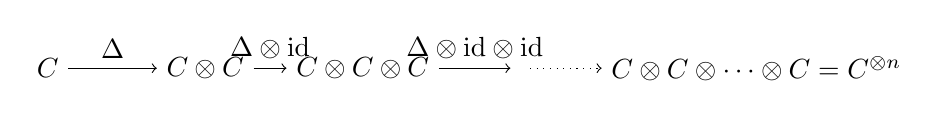
\begin{tikzpicture}
          \node (C) at (0,0) {$C$};
          \node (CC) at (2,0) {$C\otimes C$};
          \node (CCC) at (4,0) {$C\otimes C \otimes C$};
          \node (B) at (6,0) {};
          \node (NC) at (9,0) {$C\otimes C\otimes\cdots\otimes C = C^{\otimes n}$};
          \draw[->] (C) to node[above]{$\Delta$} (CC);
          \draw[->] (CC) to node[above]{$\Delta\otimes\text{id}$} (CCC);
          \draw[->] (CCC) to node[above]{$\Delta\otimes\text{id}\otimes\text{id}$} (B);
          \draw[dotted,->] (B) to node[above]{} (NC);
        \end{tikzpicture}
      \end{center}
      を合成した写像を$\Delta^{(n-1)}:C\to C^{\otimes n}$と書く.
      $\Delta^{(0)}=id,\Delta^{(1)}=\Delta$である.
    \end{remark}
    $U_q$に対しては次の公式が成り立つ.
    \begin{align*}
      \Delta^{(n-1)}(X^+) &= \sum_{j=0}^{n-1}K^{\otimes j}\otimes X^+\otimes 1^{\otimes n-j-1}\\
      \Delta^{(n-1)}(X^-) &= \sum_{j=0}^{n-1}1^{\otimes j}\otimes X^-\otimes {K^{-1}}^{\otimes n-j-1}
    \end{align*}
  \end{frame}
  \begin{frame}
    \[
    \Delta^{(1)}(X^+) = X^+\otimes 1 + K\otimes X^+ = \sum_{j=0}^{1}K^{\otimes j}\otimes X^+\otimes 1^{\otimes 1-j}
    \]
    となり,$n=1$のとき成り立つ.
    \begin{align*}
      (\Delta\otimes\text{id}^{\otimes n-1})&\Delta^{(n-1)}(X^+)\\
      &= (\Delta\otimes\text{id}^{\otimes n-1})\left(\sum_{j=0}^{n-1}K^{\otimes j}\otimes X^+\otimes 1^{\otimes n-j-1}\right)\\
      &= (\Delta\otimes\text{id}^{\otimes n-1})\left(X^+\otimes 1^{\otimes n-1} + \sum_{j=1}^{n-1}K^{\otimes j}\otimes X^+\otimes 1^{\otimes n-j-1}\right)\\
      &= (\Delta(X^+)\otimes 1^{\otimes n-1}) + \sum_{j=1}^{n-1}\Delta(K)\otimes K^{\otimes j-1}\otimes X^+\otimes 1^{\otimes n-j-1}\\
      &= (X^+\otimes 1 + K\otimes X^+)\otimes1^{\otimes n-1} + \sum_{j=1}^{n-1}K^{\otimes j+1}\otimes X^+\otimes 1^{\otimes n-j-1}\\
      &= X^+\otimes 1^{\otimes n} + K\otimes X^+\otimes 1^{\otimes n-1} + \sum_{j=1}^{n-1}K^{\otimes j+1}\otimes X^+\otimes 1^{\otimes n-j-1}
    \end{align*}
  \end{frame}
  \begin{frame}
    よって帰納的に$n$について成り立つ.
    \begin{align*}
      (\Delta\otimes\text{id}^{\otimes n-1})&\Delta^{(n-1)}(X^+)\\
      &= \sum_{j=0}^{n}K^{\otimes j}\otimes X^+\otimes 1^{\otimes n-j}
    \end{align*}
    $U_q$の対合射$S$を発見的に定義する.

    対合射の定義式に,$U_q$の生成元を代入して考える.
    \begin{align*}
      m(S\otimes\text{id})\Delta(K) &= S(K)K & u \varepsilon(K)=1\\
      m(S\otimes\text{id})\Delta(X^+) &= S(X^+)1 + S(K)X^+ & u \varepsilon(X^+)=0\\
      m(S\otimes\text{id})\Delta(X^-) &= S(X^-)K^{-1} + S(1)X^- & u \varepsilon(X^-)=0
    \end{align*}
    これにより,
    \[
    S(K)=K^{-1},\quad S(X^+)=-K^{-1}X^+,\quad S(X^-)=-X^-K
    \]
    でなくてはならない.
  \end{frame}
\end{document}
